\documentclass{beamer}
\usepackage{relsize}
\usepackage{color}

\usepackage{listings}
\usetheme{CambridgeUS}
%\usepackage{beamerthemesplit} % new 
\usepackage{enumitem}
\usepackage{amsmath}                    % See geometry.pdf to learn the layout options. 
\usepackage{amsthm}                   % See geometry.pdf to learn the layout options. There 
\usepackage{amssymb}                    % See geometry.pdf to learn the layout options. 
\usepackage[utf8]{inputenc} 
\usepackage{graphicx}
\usepackage[english,bulgarian]{babel}

\lstset{language=C++,
                basicstyle=\ttfamily,
                keywordstyle=\color{blue}\ttfamily,
                stringstyle=\color{red}\ttfamily,
                commentstyle=\color{green}\ttfamily,
                morecomment=[l][\color{magenta}]{\#}
}

\newtheorem{mydef}{Дефиниция}[section]
\newtheorem{lem}{Лема}[section]
\newtheorem{thm}{Твърдение}[section]

\DeclareMathOperator{\restrict}{\upharpoonright}

\setitemize{label=\usebeamerfont*{itemize item}%
  \usebeamercolor[fg]{itemize item}
  \usebeamertemplate{itemize item}}

\setbeamercovered{transparent}



\begin{document}
\title[Обектно ориентирано програмиране]{Наследяване. Базови сведения} 
\author{Калин Георгиев} 
\frame{\titlepage} 

\section{Споделяне на памет} 


\begin{frame}
\centerline{Моделиране на различни обекти с общи свойства}
\end{frame}


\begin{frame}[fragile]
\frametitle{Еднакви и различни}

\begin{center}
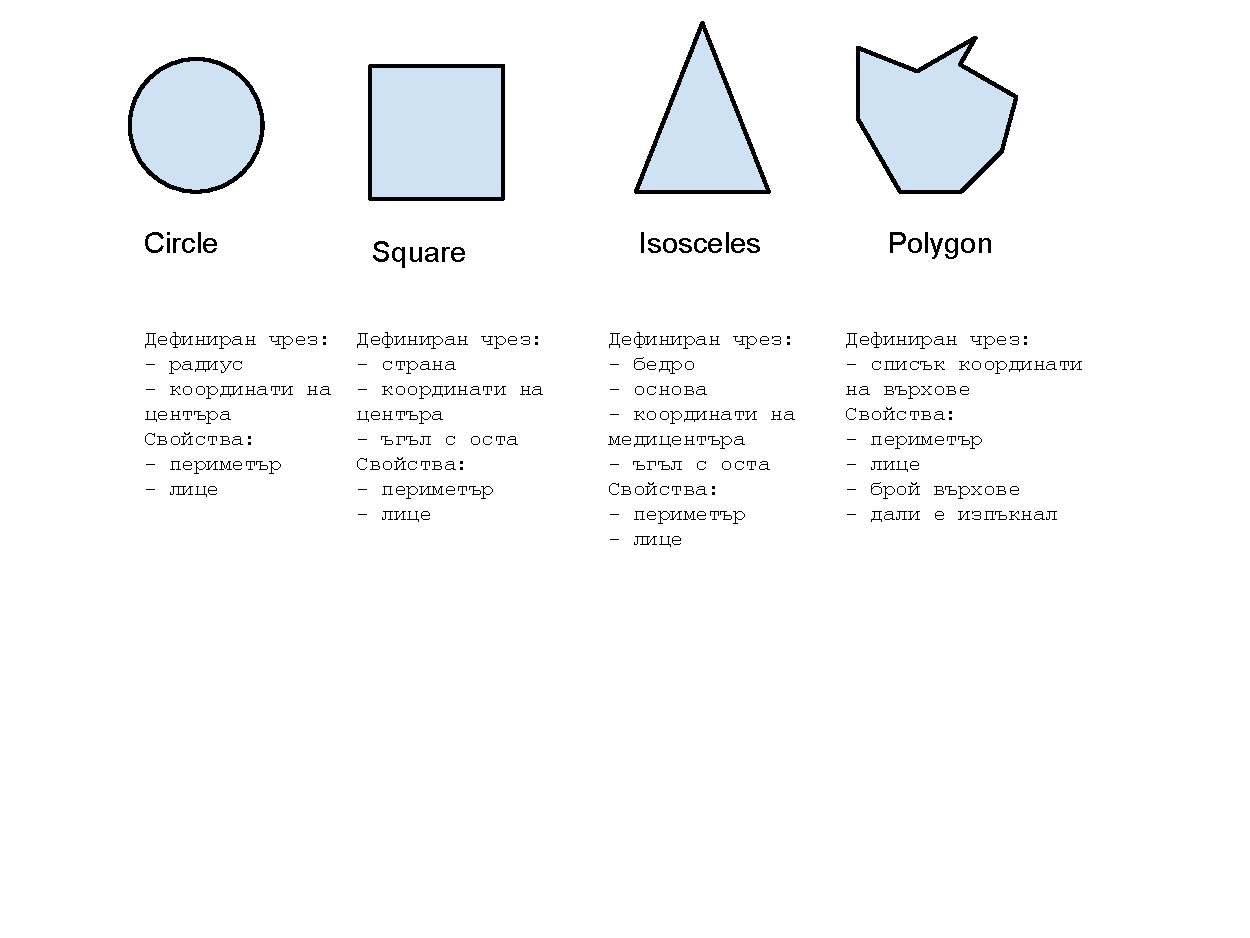
\includegraphics[width=12.0cm]{images/figures}
\end{center}


\end{frame}



\begin{frame}[fragile]
\frametitle{Множество от различни обекти}


\begin{columns}[t]
  \begin{column}{0.5\textwidth}
\begin{flushleft}
\relscale{0.6}
\begin{lstlisting}
int main ()
{
  Square* squares[] =  
     {new Square (2,0,0,0), 
      new Square (4,0,0,0),
      new Square (3,0,0,0)};

  Circle* circles[] =  
     {new Circle (2,0,0), 
      new Circle (4,0,0)};

  cout << sumSurf<Square> (squares,3) +
          sumSurf<Circle> (circles,2);

  return 0;
}
\end{lstlisting}  
\end{flushleft}
  \end{column}
  \begin{column}{0.5\textwidth}


\begin{flushleft}
\relscale{0.6}
\begin{lstlisting}
template <typename F>
double sumSurf (F* figures[], int n)
{
  double sum = 0;
  
  for (int i = 0; i < n; i++)
    sum += figures[i]->surface();

  return sum;
}
\end{lstlisting}  
\end{flushleft}

  \end{column}
\end{columns}


\end{frame}


\begin{frame}
\centerline{"Абстрахиране" от конкретния тип}
\end{frame}



\begin{frame}[fragile]
\frametitle{Какво е фигура? Йерархия от фигури}

\begin{center}
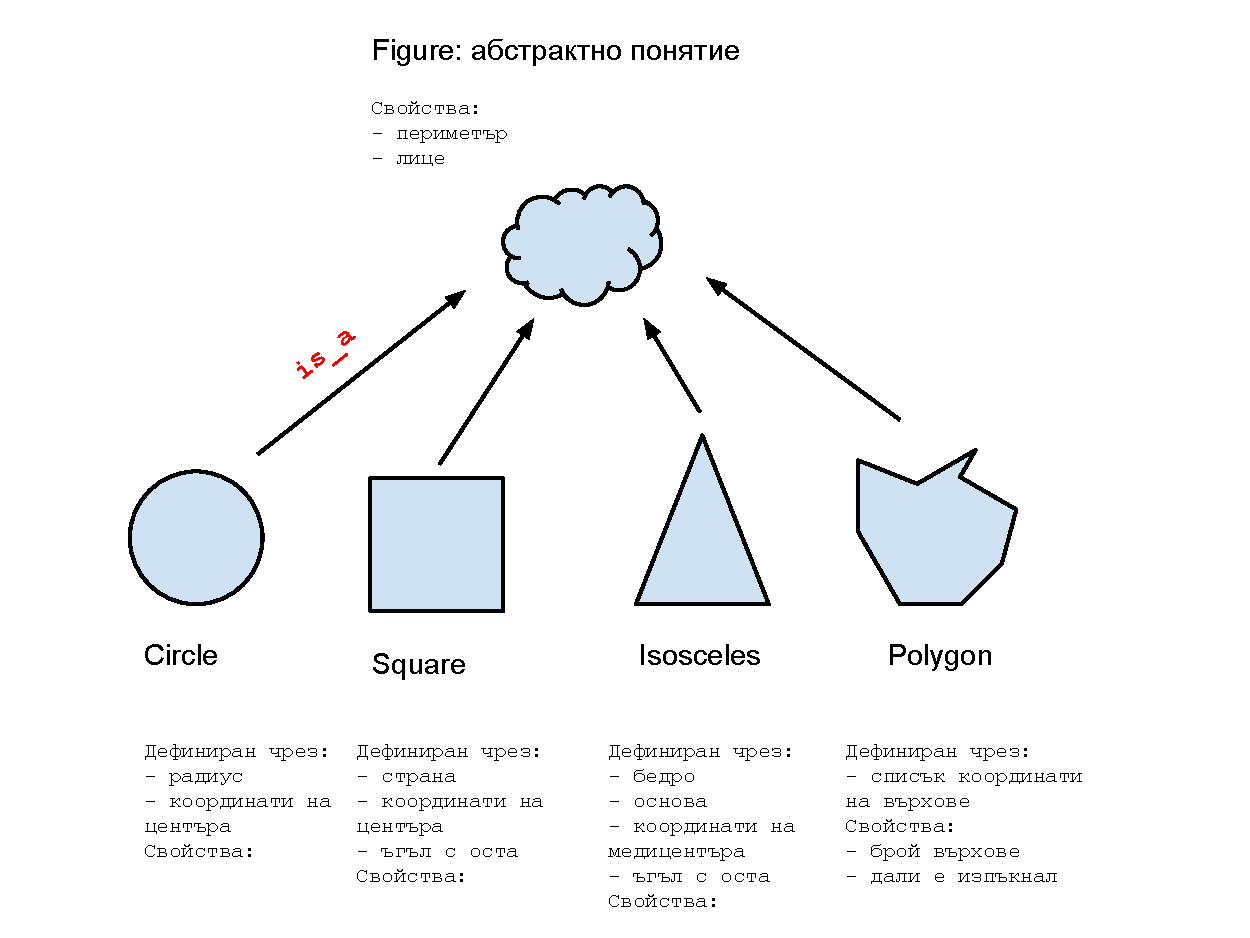
\includegraphics[width=10.0cm]{images/figures_figure} 
\end{center}

\end{frame}


\begin{frame}[fragile]
\frametitle{Полиморфизъм}


\begin{columns}[t]
  \begin{column}{0.5\textwidth}
\begin{flushleft}
\relscale{0.7}
\begin{lstlisting}
int main ()
{
  Figure* figures[] =  
     {new Square (2,0,0,0), 
      new Circle (2,0,0), 
      new Square (4,0,0,0),
      new Square (3,0,0,0),
      new Circle (4,0,0)};

  cout << sumSurf (figures,5);

  return 0;
}
\end{lstlisting}  
\end{flushleft}
  \end{column}
  \begin{column}{0.5\textwidth}


\begin{flushleft}
\relscale{0.7}
\begin{lstlisting}
template <typename F>
double sumSurf (F* figures[], int n)
{
  double sum = 0;
  
  for (int i = 0; i < n; i++)
    sum += figures[i]->surface();

  return sum;
}
\end{lstlisting}  
\end{flushleft}

  \end{column}
\end{columns}




\end{frame}

\begin{frame}
\centerline{Благодаря ви за вниманието!}
\end{frame}

\end{document}



\begin{columns}[t]
  \begin{column}{0.55\textwidth}

  \end{column}
  \begin{column}{0.45\textwidth}

  \end{column}
\end{columns}
